% Opciones para paquetes cargados en otros lugares
\PassOptionsToPackage{unicode}{hyperref}
\PassOptionsToPackage{hyphens}{url}
%
\documentclass[journal]{IEEEtran}
\usepackage[english]{babel}
\usepackage{amsmath,amssymb, graphicx}
\usepackage{lmodern}
\usepackage{iftex}
\ifPDFTeX
  \usepackage[T1]{fontenc}
  \usepackage[utf8]{inputenc}
  \usepackage{textcomp} % provide euro and other symbols
\else % if luatex or xetex
  \usepackage{unicode-math}
  \defaultfontfeatures{Scale=MatchLowercase}
  \defaultfontfeatures[\rmfamily]{Ligatures=TeX,Scale=1}
\fi

\usepackage{ragged2e} % Para el entorno justify


% Use upquote if available, for straight quotes in verbatim environments
\IfFileExists{upquote.sty}{\usepackage{upquote}}{}
\IfFileExists{microtype.sty}{% use microtype if available
  \usepackage[]{microtype}
  \UseMicrotypeSet[protrusion]{basicmath} % disable protrusion for tt fonts
}{}
\makeatletter
\@ifundefined{KOMAClassName}{% if non-KOMA class
  \IfFileExists{parskip.sty}{%
    \usepackage{parskip}
  }{% else
    \setlength{\parindent}{0pt}
    \setlength{\parskip}{6pt plus 2pt minus 1pt}}
}{% if KOMA class
  \KOMAoptions{parskip=half}}
\makeatother
\usepackage{xcolor}
\setlength{\emergencystretch}{3em} % prevent overfull lines
\providecommand{\tightlist}{%
  \setlength{\itemsep}{0pt}\setlength{\parskip}{0pt}}
\setcounter{secnumdepth}{3} % remove section numbering
\ifLuaTeX
  \usepackage{selnolig}  % disable illegal ligatures
\fi
\IfFileExists{bookmark.sty}{\usepackage{bookmark}}{\usepackage{hyperref}}
\IfFileExists{xurl.sty}{\usepackage{xurl}}{} % add URL line breaks if available
\urlstyle{same} % disable monospaced font for URLs
\hypersetup{
  hidelinks,
  pdfcreator={LaTeX via pandoc}}

\usepackage{fancyhdr}
\pagestyle{fancy}
\fancyhf{}
\renewcommand{\headrulewidth}{0pt}
\renewcommand{\footrulewidth}{0pt}
\fancyhead[R]{\scriptsize\thepage}

\newenvironment{customfontsize}{
    \fontsize{12}{14}\selectfont
}{}

\author{}
\date{}

\begin{document}
\onecolumn
\thispagestyle{empty} % Eliminar numeración en la primera página

\begin{center}
%\textbf{\fontsize{14}{16}\selectfont UNIVERSIDAD SAN FRANCISCO DE QUITO USFQ}\\
%\vspace{40pt}
%\textbf{\fontsize{14}{16}\selectfont Colegio de Posgrados}\\
%\vspace{90pt}
%\textbf{\fontsize{14}{16}\selectfont \textcolor{red}{Título del Trabajo de Titulación}}\\
%\vspace{60pt}
%\textbf{\fontsize{14}{16}\selectfont \textcolor{red}{Proyecto de Titulación}}\\
%\vspace{90pt}
%\textbf{\fontsize{18}{20}\selectfont \textcolor{red}{Nombre del autor}}\\
%\vspace{70pt}
%\textbf{\fontsize{16}{18}\selectfont \textcolor{red}{Felipe Grijalva, Ph.D.}}\\
%\vspace{15pt}
%\textbf{\fontsize{16}{18}\selectfont Director de Trabajo de Titulación}\\
%\vspace{90pt}
%\fontsize{12}{14}\selectfont Trabajo de titulación de posgrado presentado como requisito para la obtención del título de \textcolor{red}{Magíster en Inteligencia Artificial}
%\vspace{40pt}
\end{center}

%\begin{center}
%\fontsize{12}{14}\selectfont \textcolor{red}{Quito, 02 de diciembre de 2024}
%\end{center}

%\newpage

%\begin{center}
%\textbf{\fontsize{18}{16}\selectfont UNIVERSIDAD SAN FRANCISCO DE QUITO USFQ}\\
%\vspace{10pt}
%\textbf{\fontsize{18}{16}\selectfont COLEGIO DE POSGRADOS}\\
%\vspace{20pt}
%\textbf{\fontsize{14}{16}\selectfont HOJA DE APROBACIÓN DE TRABAJO DE TITULACIÓN}\\
%\vspace{10pt}
%\textbf{\fontsize{14}{16}\selectfont \textcolor{red}{Título Trabajo de Titulación}}\\
%\vspace{10pt}
%\textbf{\fontsize{14}{16}\selectfont \textcolor{red}{Nombre del estudiante}}
%\end{center}
%\vspace{20pt}

%\begin{customfontsize}
%Nombre del Director del Programa:\hspace{3cm}\textcolor{red} {Felipe Grijalva}\\
%Título académico:\hspace{6.2cm}\textcolor{red}{Ph.D. en Ingeniería Eléctrica}\\
%Director del programa de:\hspace{4.7cm}\textcolor{red}{ Inteligencia Artificial}
%\vspace{30pt}
%\\Nombre del Decano del colegio Académico:\hspace{1.6cm}\textcolor{red}{Eduardo Alba}\\ 
%Título académico:\hspace{6.2cm}\textcolor{red}{Doctor en Ciencias Matemáticas}\\
%Decano del Colegio:\hspace{5.8cm}\textcolor{red}{Ciencias e Ingenierías}
%\vspace{30pt}
%\\Nombre del Decano del Colegio de Posgrados:\hspace{1cm}\textcolor{red}{Dario Niebieskikwiat}\\
%Título académico:\hspace{6.1cm}\textcolor{red}{Doctor en Física}

%\end{customfontsize}

%\begin{center}
%\vspace{350pt}
%\textbf{\fontsize{14}{16}\selectfont Quito, \textcolor{red}{diciembre 2024}}
%\end{center}

%\newpage
%\begin{center}
%\textbf{\fontsize{14}{16}\selectfont © DERECHOS DE AUTOR}\\
%\vspace{10pt}
%\end{center}
%\begin{justify}


%\fontsize{12}{14}\selectfont
%{
%\setlength{\parindent}{3em}
%\hspace{1pt}

%Por medio del presente documento certifico que he leído todas las Políticas y Manuales de la Universidad San Francisco de Quito USFQ, incluyendo la Política de Propiedad Intelectual USFQ, y estoy de acuerdo con su contenido, por lo que los derechos de propiedad intelectual del presente trabajo quedan sujetos a lo dispuesto en esas Políticas.

%Asimismo, autorizo a la USFQ para que realice la digitalización y publicación de este trabajo en el repositorio virtual, de conformidad a lo dispuesto en la Ley Orgánica de Educación Superior del Ecuador.
%}
%\end{justify}

%\begin{customfontsize}
%\vspace{30pt}

%Nombre del estudiante:\hspace{4cm}\textcolor{red}  {\_\_\_\_\_\_\_\_\_\_\_\_\_\_\_\_\_\_\_\_\_\_\_\_\_}\\
%\vspace{30pt}

%Código de estudiante:\hspace{4.2cm}\textcolor{red}%{\_\_\_\_\_\_\_\_\_\_\_\_\_\_\_\_\_\_\_\_\_\_\_\_\_}\\
%\vspace{30pt}

%C.I.:\hspace{7.3cm}\textcolor{red}{\_\_\_\_\_\_\_\_\_\_\_\_\_\_\_\_\_\_\_\_\_\_\_\_\_}\\
%\vspace{30pt}

%Lugar y fecha:\hspace{5.4cm}\textcolor{red}{Ciudad, día} de \textcolor{red}{mes} de \textcolor{red}{año.}

%\end{customfontsize}


%\newpage

%\begin{center}
%\textbf{\fontsize{14}{16}\selectfont ACLARACIÓN PARA PUBLICACIÓN}\\
%\end{center}
%\vspace{10pt}

%\begin{justify}
%\fontsize{12}{14}\selectfont \textbf{Nota:} El presente trabajo, en su totalidad o cualquiera de sus partes, no debe ser considerado como una publicación, incluso a pesar de estar disponible sin restricciones a través de un repositorio institucional. Esta declaración se alinea con las prácticas y recomendaciones presentadas por el Committee on Publication Ethics COPE descritas por Barbour et al. (2017) Discussion document on best practice for issues around theses publishing, disponible en \url{http://bit.ly/COPETheses}.
%\end{justify}   
%\vspace{10pt}
%\begin{center}
%\textbf{\fontsize{14}{16}\selectfont UNPUBLISHED DOCUMENT}\\
%\end{center}
%\vspace{10pt}
%\begin{justify}
%\fontsize{12}{14}\selectfont \textbf{Note:} The following graduation project is available through Universidad San Francisco de Quito USFQ institutional repository. Nonetheless, this project -- in whole or in part -- should not be considered a publication. This statement follows the recommendations presented by the Committee on Publication Ethics COPE described by Barbour et al. (201
%7) Discussion document on best practice for issues around theses publishing available on \url{http://bit.ly/COPETheses}.
%\end{justify}

%\newpage

%\begin{center}
%\textbf{\fontsize{14}{16}\selectfont DEDICATORIA}\\
%\end{center}
%\vspace{10pt}
%\begin{justify}

%{
%\setlength{\parindent}{3em}
%\hspace{1pt}
%\fontsize{12}{14}\selectfont 

%\textcolor{red}{En texto normal. Debe ser redactado de manera sobria y concisa (Opcional).}

%}
%\end{justify}
%\newpage


%\begin{center}
%\textbf{\fontsize{14}{16}\selectfont AGRADECIMIENTOS}\\
%\end{center}
%\vspace{10pt}
%\fontsize{12}{14}\selectfont 

%{
%\setlength{\parindent}{3em}
%\hspace{1pt}

%\textcolor{red}{En texto normal, debe ser redactado de manera sobria y concisa. Esta sección es opcional, pero es en la que deben ir mencionadas todas las personas e instituciones que contribuyeron al desarrollo del trabajo de titulación. De igual forma, aquí debe reconocerse de manera clara y explícita a las personas naturales o jurídicas que trabajaron con el autor en la generación, colección o análisis de los datos y que deben ser reconocidos como coautores.}


%}
%\newpage

%\begin{center}
%\textbf{\fontsize{14}{16}\selectfont RESUMEN}\\
%\vspace{10pt}
%\end{center}
%\fontsize{12}{14}\selectfont 
%{
%\setlength{\parindent}{3em}
%\hspace{1pt}
%\textcolor{red}{En texto normal, se debe presentar una descripción completa pero concisa del trabajo, que motive a potenciales lectores a revisarlo por completo. El resumen debe indicar claramente cuál es el asunto tratado, haciendo referencia a las motivaciones y enfoques utilizados para su desarrollo, los resultados más destacables y las principales conclusiones que indiquen las implicaciones actuales y perspectivas futuras del asunto.}\\
%}
%\vspace{10pt}
%\begin{center}  
%\textbf{\fontsize{12}{14}\selectfont Palabras clave:} \textcolor{red}{deben incluir entre 5 y 10 palabras claves que describan el trabajo.}
%\end{center}

%\newpage

%\begin{center}
%\textbf{\fontsize{14}{16}\selectfont ABSTRACT}\\
%\end{center}
%\vspace{10pt}
%\fontsize{12}{14}\selectfont 
%{
%\setlength{\parindent}{3em}
%\hspace{1pt}
%\textcolor{red}{En texto normal, debe ser una traducción al inglés precisa del resumen.}\\

%}
%\vspace{10pt}
%\begin{center}
%\textbf{\fontsize{12}{14}\selectfont Key words:} \textcolor{red}{Presentar una traducción precisa de las palabras clave.}
%\end{center}


%\newpage

%\begin{center}
%\textbf{\fontsize{14}{16}\selectfont TABLA DE CONTENIDO}
%\end{center}

%\renewcommand{\contentsname}{}
%\begin{customfontsize}
%    \tableofcontents
%\end{customfontsize}


%\newpage

%\begin{center}
%    \textbf{\fontsize{14}{16}\selectfont ÍNDICE DE TABLAS}
%\end{center}

%\fontsize{12}{14}\selectfont TABLA \#. TÍTULO DE LA TABLA (EL TÍTULO DE LA TABLA DEBE SER AUTODESCRIPTIVO Y NO DEBE DEPENDER DEL TEXTO)

%\renewcommand{\listtablename}{} % Remove "List of Tables" title

%\begin{customfontsize}
%    \listoftables
%\end{customfontsize}


%\newpage
%\begin{center}
%    \textbf{\fontsize{14}{16}\selectfont ÍNDICE DE FIGURAS}
%\end{center}

%\fontsize{12}{14}\selectfont FIGURA \#. TÍTULO DE LA FIGURA (EL TÍTULO DEBE SER AUTODESCRIPTIVO Y NO DEBE DEPENDER DEL TEXTO)

%\renewcommand{\listfigurename}{} % Remove "List of Tables" title


%\begin{customfontsize}
%    \listoffigures
%\end{customfontsize}

\newpage
\twocolumn
%% bare_jrnl.tex
%% V1.4b
%% 2015/08/26
%% by Michael Shell
%% see http://www.michaelshell.org/
%% for current contact information.
%%
%% This is a skeleton file demonstrating the use of IEEEtran.cls
%% (requires IEEEtran.cls version 1.8b or later) with an IEEE
%% journal paper.
%%
%% Support sites:
%% http://www.michaelshell.org/tex/ieeetran/
%% http://www.ctan.org/pkg/ieeetran
%% and
%% http://www.ieee.org/

%%*************************************************************************
%% Legal Notice:
%% This code is offered as-is without any warranty either expressed or
%% implied; without even the implied warranty of MERCHANTABILITY or
%% FITNESS FOR A PARTICULAR PURPOSE! 
%% User assumes all risk.
%% In no event shall the IEEE or any contributor to this code be liable for
%% any damages or losses, including, but not limited to, incidental,
%% consequential, or any other damages, resulting from the use or misuse
%% of any information contained here.
%%
%% All comments are the opinions of their respective authors and are not
%% necessarily endorsed by the IEEE.
%%
%% This work is distributed under the LaTeX Project Public License (LPPL)
%% ( http://www.latex-project.org/ ) version 1.3, and may be freely used,
%% distributed and modified. A copy of the LPPL, version 1.3, is included
%% in the base LaTeX documentation of all distributions of LaTeX released
%% 2003/12/01 or later.
%% Retain all contribution notices and credits.
%% ** Modified files should be clearly indicated as such, including  **
%% ** renaming them and changing author support contact information. **
%%*************************************************************************


% *** Authors should verify (and, if needed, correct) their LaTeX system  ***
% *** with the testflow diagnostic prior to trusting their LaTeX platform ***
% *** with production work. The IEEE's font choices and paper sizes can   ***
% *** trigger bugs that do not appear when using other class files.       ***                          ***
% The testflow support page is at:
% http://www.michaelshell.org/tex/testflow/

%
% If IEEEtran.cls has not been installed into the LaTeX system files,
% manually specify the path to it like:
% \documentclass[journal]{../sty/IEEEtran}


% Some very useful LaTeX packages include:
% (uncomment the ones you want to load)


% *** MISC UTILITY PACKAGES ***
%
%\usepackage{ifpdf}
% Heiko Oberdiek's ifpdf.sty is very useful if you need conditional
% compilation based on whether the output is pdf or dvi.
% usage:
% \ifpdf
%   % pdf code
% \else
%   % dvi code
% \fi
% The latest version of ifpdf.sty can be obtained from:
% http://www.ctan.org/pkg/ifpdf
% Also, note that IEEEtran.cls V1.7 and later provides a builtin
% \ifCLASSINFOpdf conditional that works the same way.
% When switching from latex to pdflatex and vice-versa, the compiler may
% have to be run twice to clear warning/error messages.


% *** CITATION PACKAGES ***
%
%\usepackage{cite}
% cite.sty was written by Donald Arseneau
% V1.6 and later of IEEEtran pre-defines the format of the cite.sty package
% \cite{} output to follow that of the IEEE. Loading the cite package will
% result in citation numbers being automatically sorted and properly
% "compressed/ranged". e.g., [1], [9], [2], [7], [5], [6] without using
% cite.sty will become [1], [2], [5]--[7], [9] using cite.sty. cite.sty's
% \cite will automatically add leading space, if needed. Use cite.sty's
% noadjust option (cite.sty V3.8 and later) if you want to turn this off
% such as if a citation ever needs to be enclosed in parenthesis.
% cite.sty is already installed on most LaTeX systems. Be sure and use
% version 5.0 (2009-03-20) and later if using hyperref.sty.
% The latest version can be obtained at:
% http://www.ctan.org/pkg/cite
% The documentation is contained in the cite.sty file itself.


% *** GRAPHICS RELATED PACKAGES ***
%
\ifCLASSINFOpdf
  % \usepackage[pdftex]{graphicx}
  % declare the path(s) where your graphic files are
  % \graphicspath{{../pdf/}{../jpeg/}}
  % and their extensions so you won't have to specify these with
  % every instance of \includegraphics
  % \DeclareGraphicsExtensions{.pdf,.jpeg,.png}
\else
  % or other class option (dvipsone, dvipdf, if not using dvips). graphicx
  % will default to the driver specified in the system graphics.cfg if no
  % driver is specified.
  % \usepackage[dvips]{graphicx}
  % declare the path(s) where your graphic files are
  % \graphicspath{{../eps/}}
  % and their extensions so you won't have to specify these with
  % every instance of \includegraphics
  % \DeclareGraphicsExtensions{.eps}
\fi
% graphicx was written by David Carlisle and Sebastian Rahtz. It is
% required if you want graphics, photos, etc. graphicx.sty is already
% installed on most LaTeX systems. The latest version and documentation
% can be obtained at: 
% http://www.ctan.org/pkg/graphicx
% Another good source of documentation is "Using Imported Graphics in
% LaTeX2e" by Keith Reckdahl which can be found at:
% http://www.ctan.org/pkg/epslatex
%
% latex, and pdflatex in dvi mode, support graphics in encapsulated
% postscript (.eps) format. pdflatex in pdf mode supports graphics
% in .pdf, .jpeg, .png and .mps (metapost) formats. Users should ensure
% that all non-photo figures use a vector format (.eps, .pdf, .mps) and
% not a bitmapped formats (.jpeg, .png). The IEEE frowns on bitmapped formats
% which can result in "jaggedy"/blurry rendering of lines and letters as
% well as large increases in file sizes.
%
% You can find documentation about the pdfTeX application at:
% http://www.tug.org/applications/pdftex


% *** MATH PACKAGES ***
%
%\usepackage{amsmath}
% A popular package from the American Mathematical Society that provides
% many useful and powerful commands for dealing with mathematics.
%
% Note that the amsmath package sets \interdisplaylinepenalty to 10000
% thus preventing page breaks from occurring within multiline equations. Use:
%\interdisplaylinepenalty=2500
% after loading amsmath to restore such page breaks as IEEEtran.cls normally
% does. amsmath.sty is already installed on most LaTeX systems. The latest
% version and documentation can be obtained at:
% http://www.ctan.org/pkg/amsmath


% *** SPECIALIZED LIST PACKAGES ***
%
%\usepackage{algorithmic}
% algorithmic.sty was written by Peter Williams and Rogerio Brito.
% This package provides an algorithmic environment fo describing algorithms.
% You can use the algorithmic environment in-text or within a figure
% environment to provide for a floating algorithm. Do NOT use the algorithm
% floating environment provided by algorithm.sty (by the same authors) or
% algorithm2e.sty (by Christophe Fiorio) as the IEEE does not use dedicated
% algorithm float types and packages that provide these will not provide
% correct IEEE style captions. The latest version and documentation of
% algorithmic.sty can be obtained at:
% http://www.ctan.org/pkg/algorithms
% Also of interest may be the (relatively newer and more customizable)
% algorithmicx.sty package by Szasz Janos:
% http://www.ctan.org/pkg/algorithmicx


% *** ALIGNMENT PACKAGES ***
%
%\usepackage{array}
% Frank Mittelbach's and David Carlisle's array.sty patches and improves
% the standard LaTeX2e array and tabular environments to provide better
% appearance and additional user controls. As the default LaTeX2e table
% generation code is lacking to the point of almost being broken with
% respect to the quality of the end results, all users are strongly
% advised to use an enhanced (at the very least that provided by array.sty)
% set of table tools. array.sty is already installed on most systems. The
% latest version and documentation can be obtained at:
% http://www.ctan.org/pkg/array


% IEEEtran contains the IEEEeqnarray family of commands that can be used to
% generate multiline equations as well as matrices, tables, etc., of high
% quality.


% *** SUBFIGURE PACKAGES ***
%\ifCLASSOPTIONcompsoc
%  \usepackage[caption=false,font=normalsize,labelfont=sf,textfont=sf]{subfig}
%\else
%  \usepackage[caption=false,font=footnotesize]{subfig}
%\fi
% subfig.sty, written by Steven Douglas Cochran, is the modern replacement
% for subfigure.sty, the latter of which is no longer maintained and is
% incompatible with some LaTeX packages including fixltx2e. However,
% subfig.sty requires and automatically loads Axel Sommerfeldt's caption.sty
% which will override IEEEtran.cls' handling of captions and this will result
% in non-IEEE style figure/table captions. To prevent this problem, be sure
% and invoke subfig.sty's "caption=false" package option (available since
% subfig.sty version 1.3, 2005/06/28) as this is will preserve IEEEtran.cls
% handling of captions.
% Note that the Computer Society format requires a larger sans serif font
% than the serif footnote size font used in traditional IEEE formatting
% and thus the need to invoke different subfig.sty package options depending
% on whether compsoc mode has been enabled.
%
% The latest version and documentation of subfig.sty can be obtained at:
% http://www.ctan.org/pkg/subfig


% *** FLOAT PACKAGES ***
%
%\usepackage{fixltx2e}
% fixltx2e, the successor to the earlier fix2col.sty, was written by
% Frank Mittelbach and David Carlisle. This package corrects a few problems
% in the LaTeX2e kernel, the most notable of which is that in current
% LaTeX2e releases, the ordering of single and double column floats is not
% guaranteed to be preserved. Thus, an unpatched LaTeX2e can allow a
% single column figure to be placed prior to an earlier double column
% figure.
% Be aware that LaTeX2e kernels dated 2015 and later have fixltx2e.sty's
% corrections already built into the system in which case a warning will
% be issued if an attempt is made to load fixltx2e.sty as it is no longer
% needed.
% The latest version and documentation can be found at:
% http://www.ctan.org/pkg/fixltx2e


%\usepackage{stfloats}
% stfloats.sty was written by Sigitas Tolusis. This package gives LaTeX2e
% the ability to do double column floats at the bottom of the page as well
% as the top. (e.g., "\begin{figure*}[!b]" is not normally possible in
% LaTeX2e). It also provides a command:
%\fnbelowfloat
% to enable the placement of footnotes below bottom floats (the standard
% LaTeX2e kernel puts them above bottom floats). This is an invasive package
% which rewrites many portions of the LaTeX2e float routines. It may not work
% with other packages that modify the LaTeX2e float routines. The latest
% version and documentation can be obtained at:
% http://www.ctan.org/pkg/stfloats
% Do not use the stfloats baselinefloat ability as the IEEE does not allow
% \baselineskip to stretch. Authors submitting work to the IEEE should note
% that the IEEE rarely uses double column equations and that authors should try
% to avoid such use. Do not be tempted to use the cuted.sty or midfloat.sty
% packages (also by Sigitas Tolusis) as the IEEE does not format its papers in
% such ways.
% Do not attempt to use stfloats with fixltx2e as they are incompatible.
% Instead, use Morten Hogholm'a dblfloatfix which combines the features
% of both fixltx2e and stfloats:
%
% \usepackage{dblfloatfix}
% The latest version can be found at:
% http://www.ctan.org/pkg/dblfloatfix


%\ifCLASSOPTIONcaptionsoff
%  \usepackage[nomarkers]{endfloat}
% \let\MYoriglatexcaption\caption
% \renewcommand{\caption}[2][\relax]{\MYoriglatexcaption[#2]{#2}}
%\fi
% endfloat.sty was written by James Darrell McCauley, Jeff Goldberg and 
% Axel Sommerfeldt. This package may be useful when used in conjunction with 
% IEEEtran.cls'  captionsoff option. Some IEEE journals/societies require that
% submissions have lists of figures/tables at the end of the paper and that
% figures/tables without any captions are placed on a page by themselves at
% the end of the document. If needed, the draftcls IEEEtran class option or
% \CLASSINPUTbaselinestretch interface can be used to increase the line
% spacing as well. Be sure and use the nomarkers option of endfloat to
% prevent endfloat from "marking" where the figures would have been placed
% in the text. The two hack lines of code above are a slight modification of
% that suggested by in the endfloat docs (section 8.4.1) to ensure that
% the full captions always appear in the list of figures/tables - even if
% the user used the short optional argument of \caption[]{}.
% IEEE papers do not typically make use of \caption[]'s optional argument,
% so this should not be an issue. A similar trick can be used to disable
% captions of packages such as subfig.sty that lack options to turn off
% the subcaptions:
% For subfig.sty:
% \let\MYorigsubfloat\subfloat
% \renewcommand{\subfloat}[2][\relax]{\MYorigsubfloat[]{#2}}
% However, the above trick will not work if both optional arguments of
% the \subfloat command are used. Furthermore, there needs to be a
% description of each subfigure *somewhere* and endfloat does not add
% subfigure captions to its list of figures. Thus, the best approach is to
% avoid the use of subfigure captions (many IEEE journals avoid them anyway)
% and instead reference/explain all the subfigures within the main caption.
% The latest version of endfloat.sty and its documentation can obtained at:
% http://www.ctan.org/pkg/endfloat
%
% The IEEEtran \ifCLASSOPTIONcaptionsoff conditional can also be used
% later in the document, say, to conditionally put the References on a 
% page by themselves.


% *** PDF, URL AND HYPERLINK PACKAGES ***
%
%\usepackage{url}
% url.sty was written by Donald Arseneau. It provides better support for
% handling and breaking URLs. url.sty is already installed on most LaTeX
% systems. The latest version and documentation can be obtained at:
% http://www.ctan.org/pkg/url
% Basically, \url{my_url_here}.


% *** Do not adjust lengths that control margins, column widths, etc. ***
% *** Do not use packages that alter fonts (such as pslatex).         ***
% There should be no need to do such things with IEEEtran.cls V1.6 and later.
% (Unless specifically asked to do so by the journal or conference you plan
% to submit to, of course. )


% correct bad hyphenation here
\hyphenation{op-tical net-works semi-conduc-tor}

% paper title
% Titles are generally capitalized except for words such as a, an, and, as,
% at, but, by, for, in, nor, of, on, or, the, to and up, which are usually
% not capitalized unless they are the first or last word of the title.
% Linebreaks \\ can be used within to get better formatting as desired.
% Do not put math or special symbols in the title.
\title{Human Activity Recognition Using Deep Learning Models on the KU-HAR Dataset}


% author names and IEEE memberships
% note positions of commas and nonbreaking spaces ( ~ ) LaTeX will not break
% a structure at a ~ so this keeps an author's name from being broken across
% two lines.
% use \thanks{} to gain access to the first footnote area
% a separate \thanks must be used for each paragraph as LaTeX2e's \thanks
% was not built to handle multiple paragraphs
%

\author{Guillermo~Fernández,~\IEEEmembership{Student,~Master in Artificial Intelligence}
        %Oscar~Cajamarca,~\IEEEmembership{Member,~IEEE,}
        %and~Jane~Doe,~\IEEEmembership{Life~Fellow,~IEEE}% <-this % stops a space
%\thanks{F. Grijalva and O. Cajamarca are with Universidad San Francisco de Quito USFQ}% <-this % stops a space
%\thanks{J. Reinoso is a Computer Science student at USFQ, Quito, Ecuador}%<-this % stops a space
%\thanks{Manuscript received April 19, 2005; revised August 26, 2015. modified July 31, 2024.}
}

% note the % following the last \IEEEmembership and also \thanks - 
% these prevent an unwanted space from occurring between the last author name
% and the end of the author line. i.e., if you had this:
% 
% \author{....lastname \thanks{...} \thanks{...} }
%                     ^------------^------------^----Do not want these spaces!
%
% a space would be appended to the last name and could cause every name on that
% line to be shifted left slightly. This is one of those "LaTeX things". For
% instance, "\textbf{A} \textbf{B}" will typeset as "A B" not "AB". To get
% "AB" then you have to do: "\textbf{A}\textbf{B}"
% \thanks is no different in this regard, so shield the last } of each \thanks
% that ends a line with a % and do not let a space in before the next \thanks.
% Spaces after \IEEEmembership other than the last one are OK (and needed) as
% you are supposed to have spaces between the names. For what it is worth,
% this is a minor point as most people would not even notice if the said evil
% space somehow managed to creep in.


% The paper headers
%\markboth{Journal of \LaTeX\ Class Files,~Vol.~14, No.~8, August~2015}%
%{Shell \MakeLowercase{\textit{et al.}}: Bare Demo of IEEEtran.cls for IEEE Journals}
% The only time the second header will appear is for the odd numbered pages
% after the title page when using the twoside option.
% 
% *** Note that you probably will NOT want to include the author's ***
% *** name in the headers of peer review papers.                   ***
% You can use \ifCLASSOPTIONpeerreview for conditional compilation here if
% you desire.


% If you want to put a publisher's ID mark on the page you can do it like
% this:
%\IEEEpubid{0000--0000/00\$00.00~\copyright~2015 IEEE}
% Remember, if you use this you must call \IEEEpubidadjcol in the second
% column for its text to clear the IEEEpubid mark.


% use for special paper notices
%\IEEEspecialpapernotice{(Invited Paper)}
\fontsize{10}{12}\selectfont
% make the title area
\maketitle

% As a general rule, do not put math, special symbols or citations
% in the abstract or keywords.

\begin{abstract}

Human Activity Recognition (HAR) has become a new field of active research due to its applications in healthcare, sports monitoring, assisted living, and intelligent mobile systems. Recent advances in deep learning have significantly improved the ability to automatically recognize human activities from wearable devices and smartphone sensors. This work presents a comparative evaluation of three deep learning architectures for HAR using the publicly available KU-HAR dataset, which contains recordings from smartphone accelerometers and gyroscopes sensors acquired from 90 participants performing 18 different activities.

Three representative architectures were implemented and evaluated: a one-dimensional Convolutional Neural Network (CNN1D), a Bidirectional Long Short-Term Memory network (BiLSTM), and a hybrid Convolutional Recurrent Neural Network (CRNN). All models were trained under the same preprocessing pipeline and evaluated using Accuracy, Balanced Accuracy, Macro F1-score, Weighted F1-score, model complexity, and computational cost.

Experimental results show that the BiLSTM achieved the highest recognition performance, reaching a test accuracy of 97.37\% and a Macro F1-score of 98.08\%. However, this improvement required considerably longer training times. In contrast, the CNN1D presented the lowest computational cost while maintaining acceptable performance, whereas the CRNN offered a compromise between accuracy and computational efficiency. These findings highlight the trade-off between predictive performance and computational requirements when selecting deep learning models for smartphone-based HAR applications.

\end{abstract}

% Note that keywords are not normally used for peerreview papers.
\begin{IEEEkeywords}
CNN, Wearable, movement, smartphones.
\end{IEEEkeywords}

% For peer review papers, you can put extra information on the cover
% page as needed:
% \ifCLASSOPTIONpeerreview
% \begin{center} \bfseries EDICS Category: 3-BBND \end{center}
% \fi
%
% For peerreview papers, this IEEEtran command inserts a page break and
% creates the second title. It will be ignored for other modes.
\IEEEpeerreviewmaketitle



\section{Introduction}
% The very first letter is a 2 line initial drop letter followed
% by the rest of the first word in caps.
% 
% form to use if the first word consists of a single letter:
% \IEEEPARstart{A}{demo} file is ....
% 
% form to use if you need the single drop letter followed by
% normal text (unknown if ever used by the IEEE):
% \IEEEPARstart{A}{}demo file is ....
% 
% Some journals put the first two words in caps:
% \IEEEPARstart{T}{his demo} file is ....
% 
% Here we have the typical use of a "T" for an initial drop letter
% and "HIS" in caps to complete the first word.
\IEEEPARstart{H}{uman} Activity Recognition (HAR) has emerged as one of the most important research areas in artificial intelligence due to its wide range of applications in healthcare, rehabilitation, sports performance analysis, elderly assistance, human-computer interaction \cite{bulling2014,lara2013}, and smart environments. The fast expansion of smartphones equipped with inertial sensors has enabled continuous monitoring of human movements without requiring specialized hardware, making smartphone-based HAR an attractive and cost-effective solution.

Traditional machine learning approaches for HAR rely on handcrafted feature extraction followed by conventional classifiers. Although these methods have demonstrated satisfactory performance in controlled scenarios, they often require significant domain expertise and may not generalize well to complex movement patterns. Deep learning techniques overcome these limitations by automatically learning hierarchical representations directly from raw sensor signals, eliminating the need for manual feature engineering.

Among deep learning approaches, Convolutional Neural Networks (CNNs) have shown excellent capability for extracting local temporal patterns from inertial signals, while Long Short-Term Memory (LSTM) networks are particularly effective at modeling temporal dependencies present in sequential data. More recently, hybrid Convolutional Recurrent Neural Networks (CRNNs) have combined the strengths of both architectures by integrating convolutional feature extraction with recurrent temporal modeling.

Despite the increasing popularity of these models, selecting the most appropriate architecture remains a challenge because prediction accuracy must be balanced against computational cost and training time, especially for real-time applications deployed on mobile or embedded devices.

This work presents a comparative evaluation of three representative deep learning architectures for smartphone-based HAR using the KU-HAR dataset. The proposed project try to investigate the performance of a one-dimensional Convolutional Neural Network (CNN1D), a Bidirectional Long Short-Term Memory network (BiLSTM), and a Convolutional Recurrent Neural Network (CRNN). The comparison considers not only classification performance but also computational efficiency, including training time and model complexity, providing practical insights into the strengths and limitations of each architecture.






% You must have at least 2 lines in the paragraph with the drop letter
% (should never be an issue)
%I wish you the best of success.

%\hfill mds
 
%\hfill July 31, 2024

\section{Related Work}

HAR has been extensively investigated over the past decade due to the widespread availability of wearable devices and smartphones equipped with inertial sensors. Early HAR systems primarily relied on handcrafted feature extraction techniques combined with traditional machine learning classifiers such as Support Vector Machines (SVM), Decision Trees (DT), k-Nearest Neighbors (k-NN), and Random Forests (RF). Although these methods achieved satisfactory performance under controlled conditions, they required significant domain knowledge for feature engineering and often exhibited limited generalization capabilities.

The emergence of deep learning has transformed HAR by enabling end-to-end learning directly from raw sensor signals. Convolutional Neural Networks (CNNs) have demonstrated remarkable capability for automatically extracting local temporal features from multivariate time-series data while reducing the need for manual feature design. Several studies have reported that one-dimensional CNNs provide an efficient solution for smartphone-based HAR due to their relatively low computational complexity and parallel processing capabilities.

Recurrent neural networks, particularly Long Short-Term Memory (LSTM) architectures, have also become popular for HAR because they explicitly model temporal dependencies present in sequential sensor data. Bidirectional LSTM (BiLSTM) networks further improve temporal representation by simultaneously processing sequences in both forward and backward directions, allowing the model to capture contextual information from the complete activity sequence.

More recently, hybrid Convolutional Recurrent Neural Networks (CRNNs) have combined convolutional feature extraction with recurrent temporal modeling. The convolutional layers learn local motion patterns while the recurrent layers capture long-term temporal dependencies, often leading to improved recognition accuracy. However, these architectures usually require higher computational resources and longer training times than simpler CNN-based models.

Although numerous studies have reported competitive performance using these deep learning approaches, selecting the most appropriate architecture remains application-dependent. In particular, practical deployments on mobile and embedded platforms require balancing classification accuracy against computational cost, memory requirements, and training efficiency. Motivated by these considerations, this work presents a comparative evaluation of CNN1D, BiLSTM, and CRNN architectures using the KU-HAR dataset under identical preprocessing and evaluation protocols.

\section{Materials and Methods}

This section describes the dataset, preprocessing pipeline, exploratory data analysis, deep learning architectures, and experimental configuration employed throughout the study. All experiments were conducted under identical conditions to ensure a fair comparison among the evaluated models.

\subsection{KU-HAR Dataset}

The experiments were conducted using the publicly available KU-HAR (KUST Human Activity Recognition) dataset, which was specifically designed for smartphone-based human activity recognition. The dataset contains inertial measurements collected from 90 participants (75 male and 15 female) performing 18 daily activities while carrying a smartphone equipped with a tri-axial accelerometer and gyroscope.

The original dataset consists of 1,945 raw recordings that were subsequently segmented into 20,750 non-overlapping subsamples. Each subsample represents a three-second activity window sampled at 100 Hz, resulting in 300 temporal observations for each sensor channel.

Each sample contains six synchronized channels corresponding to the three accelerometer axes (X, Y, and Z) and the three gyroscope axes (X, Y, and Z). Consequently, each observation is represented by a multivariate time series of dimensions \(6 \times 300\), yielding 1,800 numerical features. Additionally, each record includes the activity label, window length, and sample identifier.

The dataset comprises eighteen activity classes, including static activities (Stand, Sit, Lay), transitional movements (Stand-Sit and Lay-Stand), locomotion activities (Walk, Run, Stair-Up, Stair-Down), and more complex dynamic actions such as Jump, Push-up, Sit-up, Pick, and Table Tennis.

\subsection{Exploratory Data Analysis}

Before model development, an exploratory data analysis was conducted to verify the integrity of the dataset, examine the distribution of activity classes, and identify relevant temporal patterns in the accelerometer and gyroscope signals. This analysis was also used to evaluate whether the sensor measurements contained sufficient discriminative information for the subsequent Human Activity Recognition experiments.

\subsubsection{Dataset Integrity}

The original KU-HAR dataset contained 20,750 activity samples and 1,803 columns. Of these columns, 1,800 corresponded to inertial sensor measurements, while the remaining three represented the activity label, sequence length, and subject identifier. Each sample contained 300 temporal observations obtained from six channels: three accelerometer axes and three gyroscope axes.

The initial inspection confirmed that the dataset contained no missing or infinite values. In addition, all activity samples were represented by sequences of 300 time steps, allowing the sensor data to be consistently reshaped into tensors of dimensions $6 \times 300$. This uniform representation was subsequently used as the input format for all deep learning architectures evaluated in this study.

\subsubsection{Class Distribution}

The distribution of samples among the eighteen activity categories was examined to identify possible class imbalance. As shown in Fig.~\ref{fig:class_distribution}, the number of observations varied considerably across classes. While several activities contained more than 1,700 samples, some categories were represented by fewer than 500 observations.

The ratio between the most represented and least represented classes was approximately 8.41. This imbalance motivated the use of class-weighted cross-entropy during model training and the inclusion of Balanced Accuracy and Macro F1-score as evaluation metrics.

\begin{figure}[ht]
    \centering
    
\includegraphics[scale=0.25]{Template_IEEE_MMIA_MSDS_USFQ/class_distribution.png}
    \caption{Distribution of samples across the eighteen activity classes in the KU-HAR dataset.}
    \label{fig:example}
\end{figure}

\subsubsection{Signal Magnitude Analysis}

To provide an orientation-independent representation of body motion, the magnitude of the accelerometer and gyroscope signals was computed from the three spatial axes. The resulting signals summarize the overall intensity of linear acceleration and angular velocity throughout each activity window.

Figures~\ref{fig:acc_mag} and~\ref{fig:gyr_mag} present representative magnitude signals extracted from the accelerometer and gyroscope, respectively. Compared with the individual sensor axes, the magnitude representation facilitates the visualization of movement intensity while reducing the influence of smartphone orientation.

Dynamic activities exhibit larger oscillations and greater signal variability, whereas static activities produce considerably more stable magnitude profiles. These observations suggest that the magnitude signals contain meaningful information that can support activity discrimination.

\begin{figure}[ht]
    \centering
    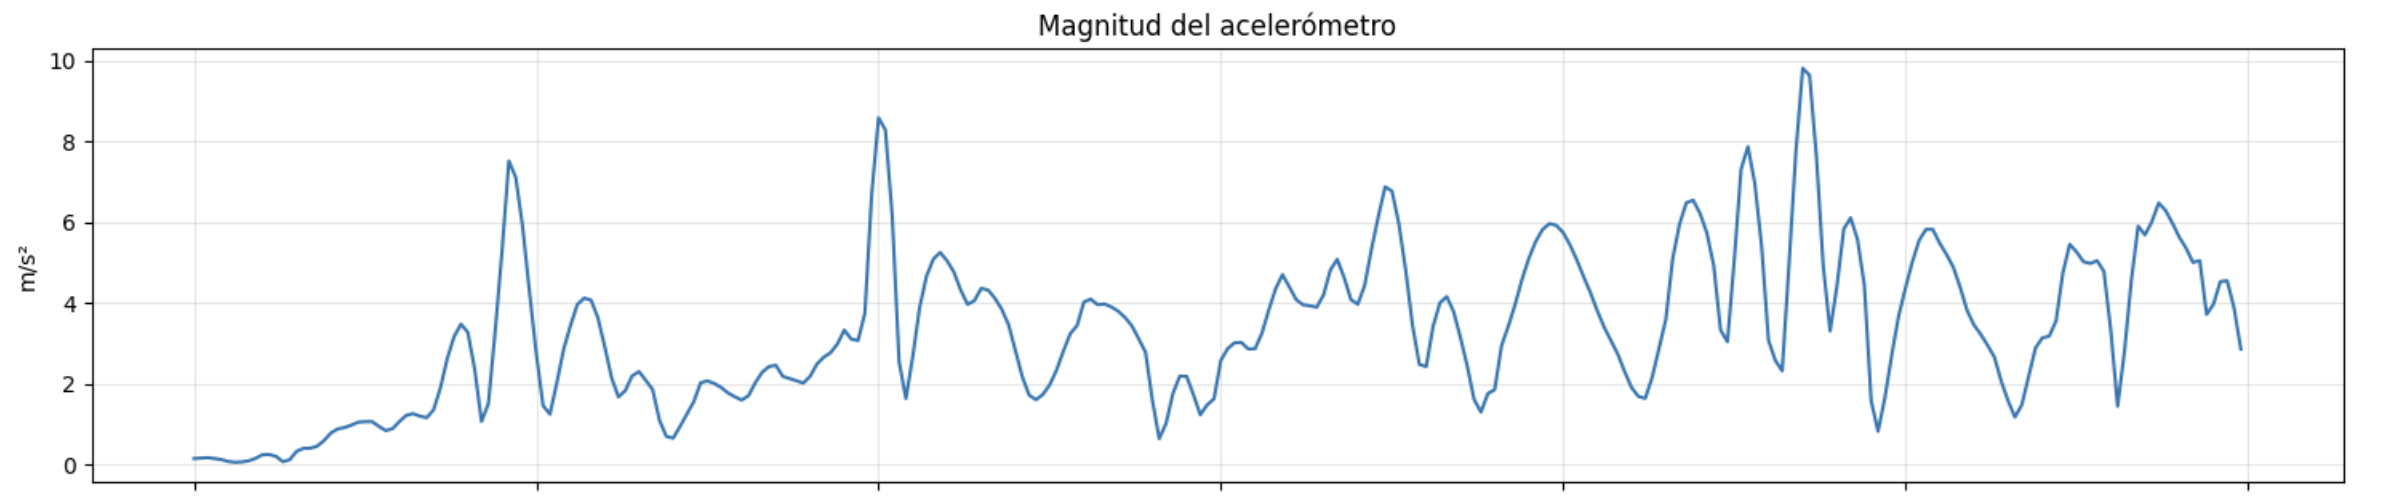
\includegraphics[scale=0.20]{accelerometer_magnitude.png}
    \caption{Representative accelerometer magnitude signals computed from the three spatial axes.}
    \label{fig:example}
\end{figure}

\begin{figure}[ht]
    \centering
    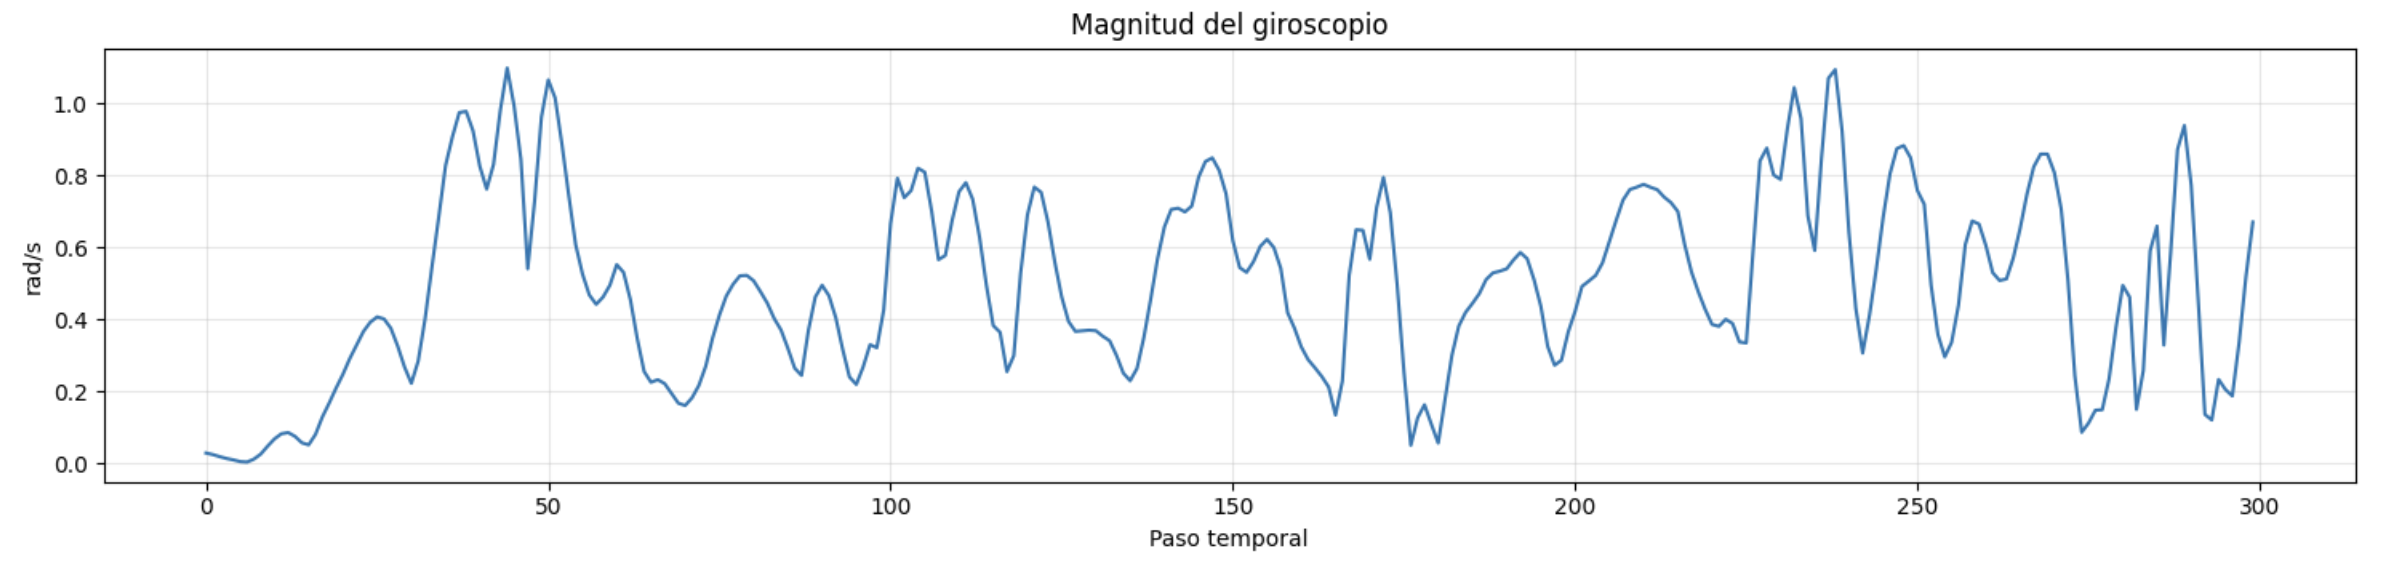
\includegraphics[scale=0.20]{gyroscope_magnitude.png}
    \caption{Representative gyroscope magnitude signals computed from the three spatial axes.}
    \label{fig:example}
\end{figure}


\subsubsection{Comparison of Activity Magnitudes}

To further investigate the separability of the recorded activities, representative magnitude signals from multiple activity classes were compared.

Static activities such as standing and sitting exhibit nearly constant magnitude profiles, while transitional movements generate localized fluctuations associated with changes in body posture. In contrast, dynamic activities including walking, running, and jumping display periodic oscillations with considerably larger amplitudes. These differences indicate that movement intensity and temporal behavior vary substantially across activity categories.

Although some activities present partially overlapping magnitude profiles, the complete six-channel sensor representation preserves additional spatial information that can be exploited by deep learning architectures to improve classification performance.

\subsubsection{Summary of the Exploratory Analysis}

The exploratory analysis confirmed the suitability of the KU-HAR dataset for Human Activity Recognition. The dataset exhibited consistent temporal windows without missing values and a manageable degree of class imbalance. Moreover, the magnitude visualizations revealed distinctive motion patterns among static, transitional, and dynamic activities, providing qualitative evidence that the inertial signals contain sufficient discriminative information for deep learning-based classification.


\subsection{Data Preprocessing}

To ensure a fair comparison among the evaluated models, a unified preprocessing pipeline was applied to all experiments.

The complete dataset was first divided into training (70\%), validation (15\%), and testing (15\%) subsets using stratified sampling to preserve the original class distribution.

Instead of conventional standardization, robust normalization was adopted to reduce the influence of extreme observations. Median and interquartile range (IQR) statistics were computed exclusively from the training subset to avoid information leakage. Each sensor channel was independently normalized according to

\begin{equation}
x'=\frac{x-\mathrm{Median}}{\mathrm{IQR}},
\end{equation}

followed by clipping the normalized values to the interval $[-10,10]$.

This strategy improves numerical stability during optimization while preserving the temporal structure of the multivariate signals. Finally, all samples were converted into tensors with dimensions \(6 \times 300\), maintaining the original synchronization among the six sensor channels.


\subsection{Deep Learning Architectures}

Three deep learning models were implemented to evaluate different strategies for learning temporal patterns from multivariate inertial sensor data. All architectures received the same input representation, consisting of six synchronized sensor channels and 300 temporal samples per activity window. The models were trained and evaluated under identical experimental conditions to ensure a fair comparison.

The evaluated architectures include a one-dimensional Convolutional Neural Network (CNN1D), a Bidirectional Long Short-Term Memory network (BiLSTM), and a hybrid Convolutional Recurrent Neural Network (CRNN). Each model represents a different approach to feature extraction and temporal modeling, allowing the analysis of their strengths and computational requirements.

\subsubsection{One-Dimensional Convolutional Neural Network}

The CNN1D model was designed to automatically learn local temporal patterns from the inertial signals through successive convolutional operations. The network consists of multiple one-dimensional convolutional layers followed by batch normalization, ReLU activation functions, max-pooling layers, and dropout regularization. The extracted feature maps are flattened and passed through fully connected layers to perform the final activity classification.

CNNs are particularly effective for HAR because neighboring samples in inertial signals often contain correlated motion information. Furthermore, one-dimensional convolutions significantly reduce computational complexity compared to recurrent architectures while maintaining competitive recognition performance.

\begin{figure}[ht]
    \centering
    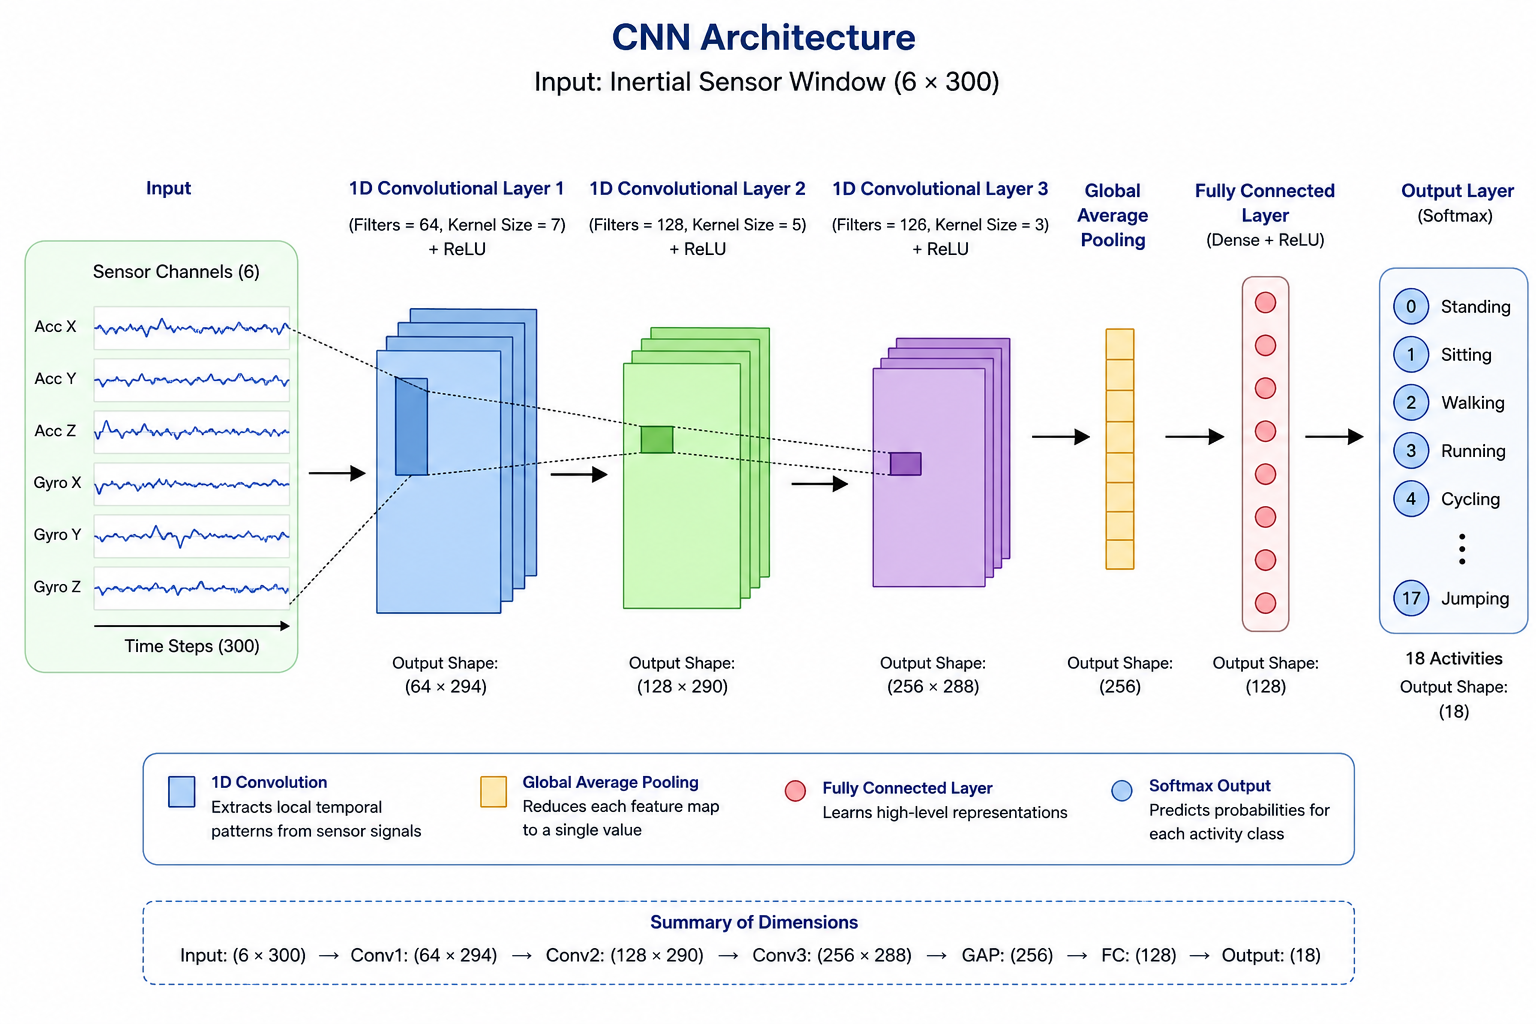
\includegraphics[scale=0.15]
    {cnn_architecture.png}
    \caption{Architecture of the proposed CNN1D model.}
    \label{fig:example}
\end{figure}


\subsection{Experimental Setup}

All experiments were implemented in Python using PyTorch and PyTorch Lightning. Training was performed using the Adam optimizer with categorical cross-entropy loss. Early stopping and model checkpointing were employed to prevent overfitting and preserve the best-performing model during training.

The dataset was divided into training (70\%), validation (15\%), and testing (15\%) subsets using stratified sampling. All models were trained using identical data partitions, ensuring a fair comparison among the evaluated architectures.

Model performance was assessed using multiple evaluation metrics, including Accuracy, Balanced Accuracy, Macro F1-score, Weighted F1-score, confusion matrices, and training time. Additionally, the number of trainable parameters was recorded to evaluate model complexity.


\begin{table}[!t]
\caption{Training Hyperparameters}
\label{tab:hyperparameters}
\centering
\begin{tabular}{lc}
\hline
Parameter & Value\\
\hline
Optimizer & Adam\\
Learning Rate & 0.001\\
Loss Function & Cross Entropy\\
Batch Size & 64\\
Epochs & 50\\
Early Stopping & Yes\\
Random Seed & 42\\
\hline
\end{tabular}
\end{table}


\section{Experimental Results}

This section presents the experimental results obtained by the CNN1D, BiLSTM, and CRNN architectures on the KU-HAR test subset. The models were evaluated using Accuracy, Balanced Accuracy, Macro F1-score, Weighted F1-score, number of trainable parameters, and training time. Learning curves and confusion matrices were also analyzed to assess convergence behavior and class-level performance.

\subsection{CNN1D Results}

The CNN1D model achieved a test accuracy of 82.78\%, a Balanced Accuracy of 88.86\%, a Macro F1-score of 89.29\%, and a Weighted F1-score of 83.38\%. The difference between the standard accuracy and the Balanced Accuracy indicates that the model performed better when each activity class was considered with equal importance.

The learning curves presented in Fig.~\ref{fig:cnn_learning_curves} show a stable reduction in both training and validation loss. Similarly, the accuracy curves improved progressively throughout training. The relatively small separation between the training and validation curves suggests that the regularization mechanisms were effective in limiting overfitting.

The CNN1D contained 260,754 trainable parameters and required approximately 181 seconds to complete training. Therefore, it represented the computationally least expensive architecture evaluated in this study.

\begin{table}[!t]
\caption{Performance of the CNN1D Model}
\label{tab:cnn_results}
\centering
\begin{tabular}{lc}
\hline
Metric & Result \\
\hline
Accuracy & 82.78\% \\
Balanced Accuracy & 88.86\% \\
Macro F1-score & 89.29\% \\
Weighted F1-score & 83.38\% \\
Trainable Parameters & 260,754 \\
Training Time & 181 s \\
\hline
\end{tabular}
\end{table}

\begin{figure}[!t]
\centering
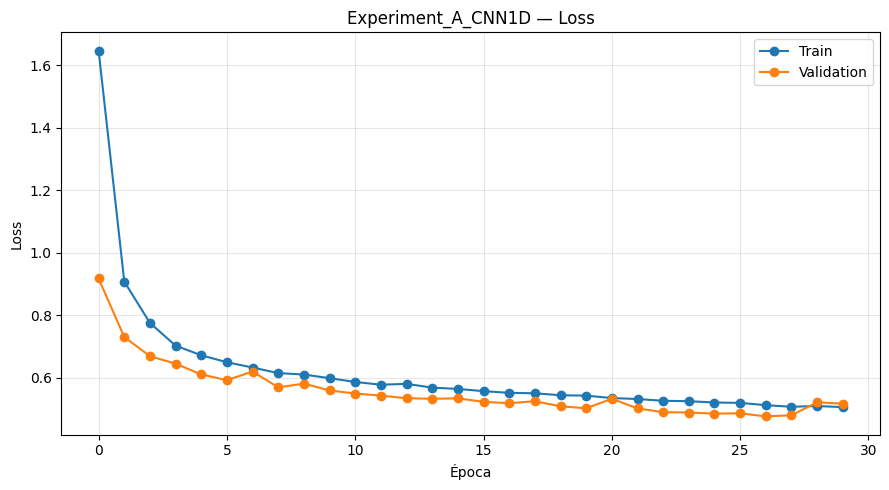
\includegraphics[width=\columnwidth]
{cnn_learning_curves.png}
\caption{Training and validation learning curves of the CNN1D model.}
\label{fig:cnn_learning_curves}
\end{figure}

\begin{figure}[!t]
\centering
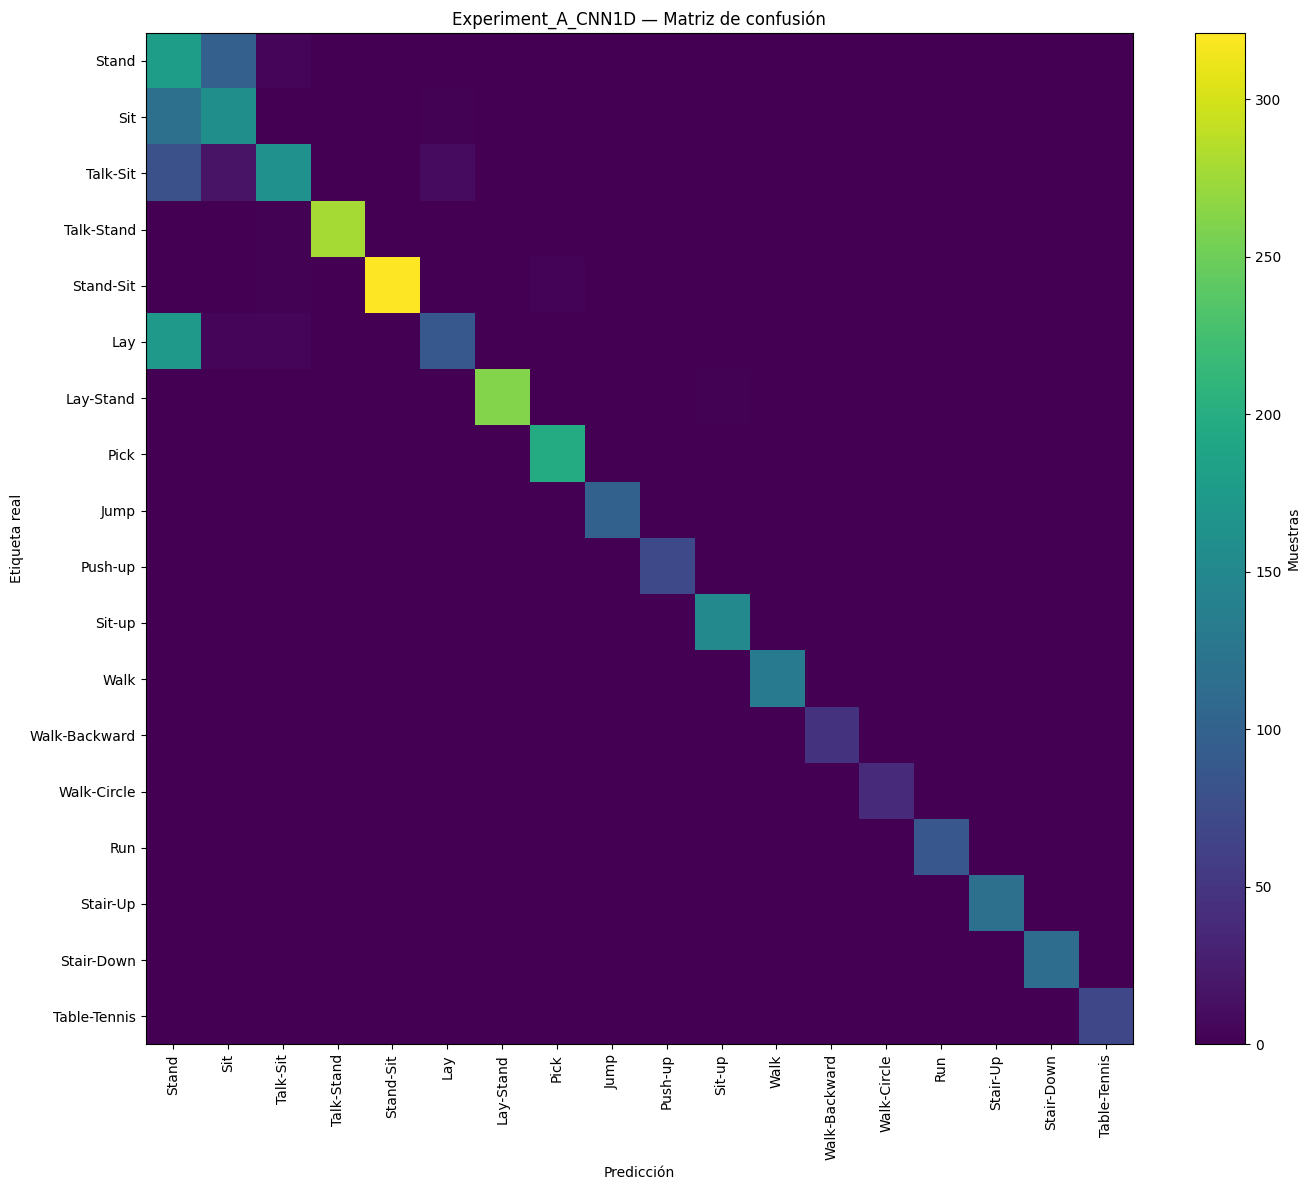
\includegraphics[width=\columnwidth]
{cnn_confusion_matrix.png}
\caption{Confusion matrix obtained by the CNN1D model on the test subset.}
\label{fig:cnn_confusion_matrix}
\end{figure}

\subsection{BiLSTM Results}

The BiLSTM obtained the highest predictive performance among the evaluated architectures, achieving a test accuracy of 97.37\% and a Macro F1-score of 98.08\%. These results demonstrate the effectiveness of bidirectional recurrent processing for modeling the temporal dependencies contained in the inertial signals.

As shown in Fig.~\ref{fig:bilstm_learning_curves}, the training and validation curves followed similar trajectories during optimization. The validation loss remained stable while the validation accuracy approached the training accuracy, indicating strong generalization and limited evidence of overfitting.

Despite its superior classification performance, the BiLSTM required approximately 1.5 hours of training. This was substantially longer than the training times recorded for the CNN1D and CRNN models. The result highlights the increased computational cost associated with recurrent processing of complete temporal sequences.

\begin{table}[!t]
\caption{Performance of the BiLSTM Model}
\label{tab:bilstm_results}
\centering
\begin{tabular}{lc}
\hline
Metric & Result \\
\hline
Accuracy & 97.37\% \\
Macro F1-score & 98.08\% \\
Test Loss & 0.274 \\
Training Time & $\approx$1.5 h \\
\hline
\end{tabular}
\end{table}

\begin{figure}[!t]
\centering
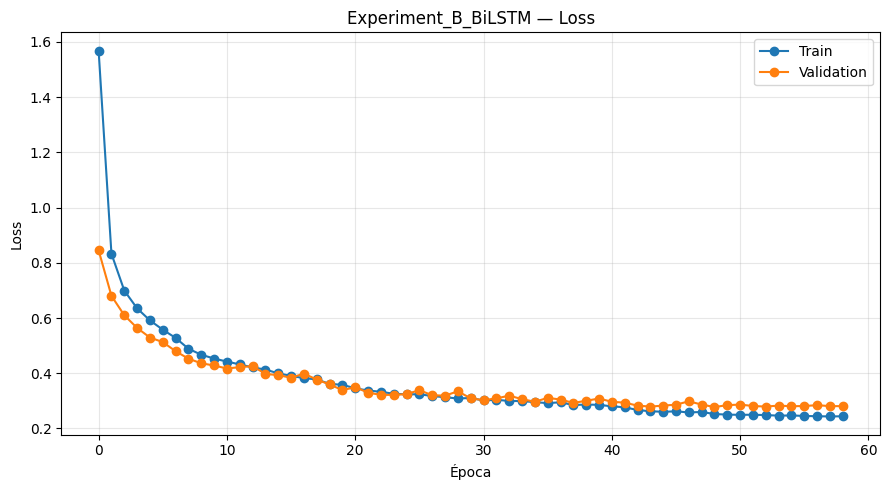
\includegraphics[width=\columnwidth]
{bilstm_learning_curves.png}
\caption{Training and validation learning curves of the BiLSTM model.}
\label{fig:bilstm_learning_curves}
\end{figure}


\begin{figure}[!t]
\centering
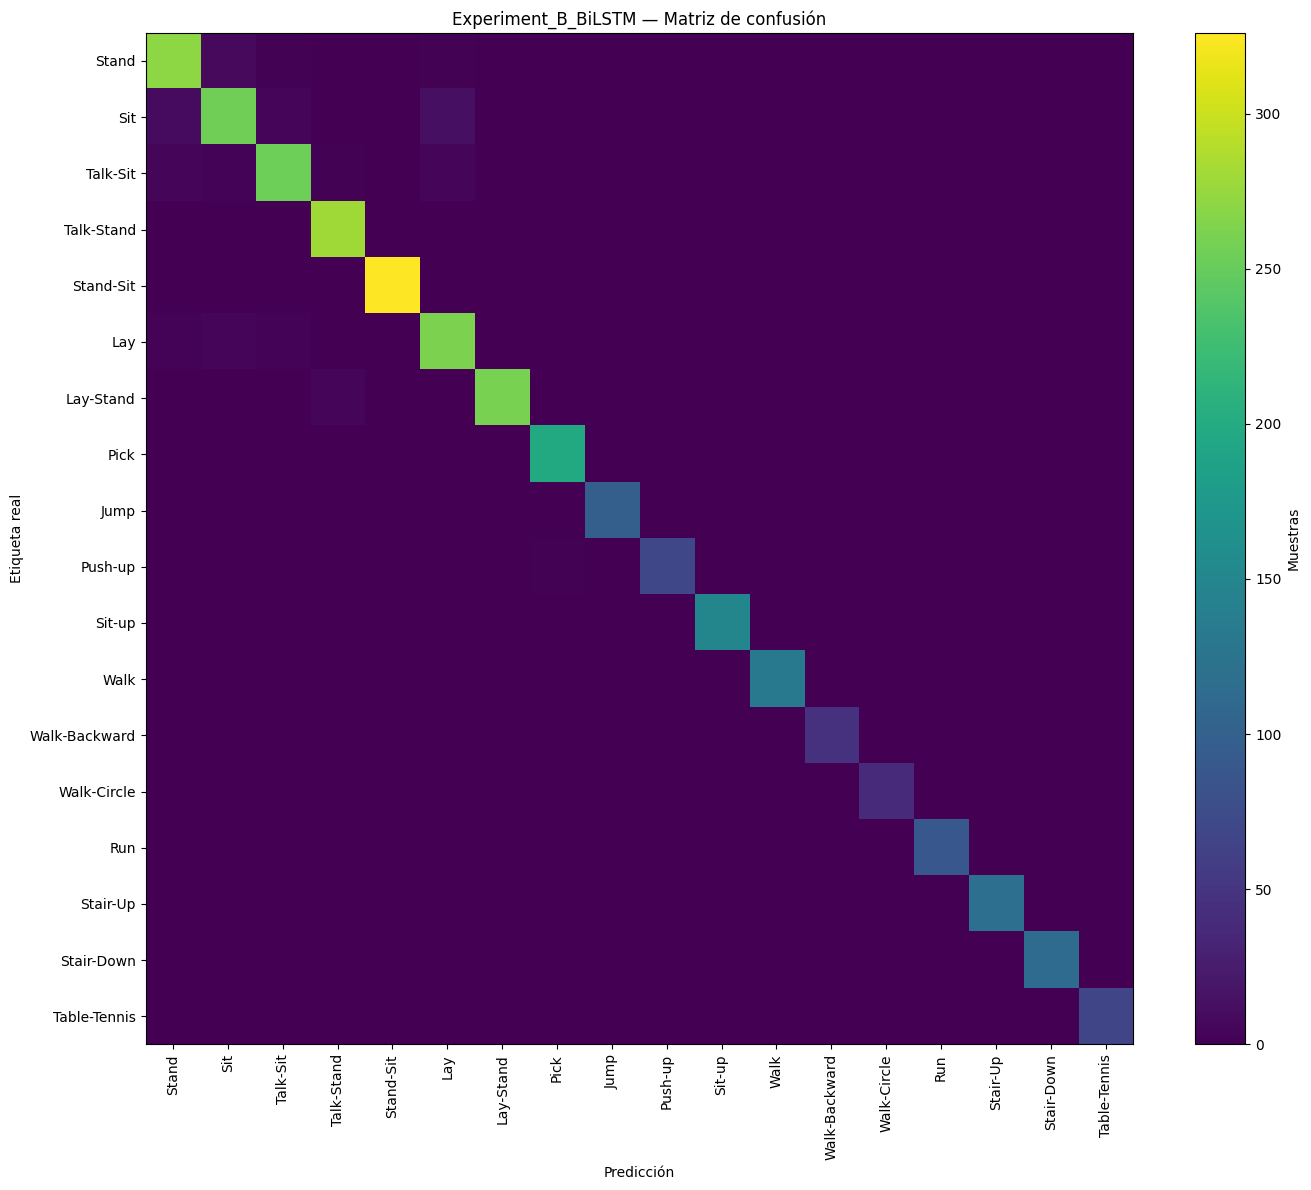
\includegraphics[width=\columnwidth]
{bilstm_confusion_matrix.png}
\caption{Confusion matrix obtained by the BiLSTM model on the test subset.}
\label{fig:bilstm_confusion_matrix}
\end{figure}

The confusion matrix presented in Fig.~\ref{fig:bilstm_confusion_matrix} confirms that the BiLSTM achieved consistent recognition across the eighteen activity classes. Only a limited number of samples were assigned to incorrect categories, indicating that bidirectional sequence modeling was effective in distinguishing both static and dynamic activities.

\subsection{CRNN Results}

The CRNN achieved a test accuracy of 85.93\%, a Balanced Accuracy of 90.76\%, a Macro F1-score of 91.00\%, and a Weighted F1-score of 86.03\%. These results represent an improvement over the CNN1D in all reported classification metrics.

The learning curves in Fig.~\ref{fig:crnn_learning_curves} demonstrate stable optimization behavior. Both training and validation performance improved progressively, although the final results remained below those obtained by the BiLSTM.

The CRNN contained 361,106 trainable parameters and required approximately seven minutes to complete training. Therefore, its computational cost was higher than that of the CNN1D but substantially lower than that of the BiLSTM.


\begin{table}[!t]
\caption{Performance of the CRNN Model}
\label{tab:crnn_results}
\centering
\begin{tabular}{lc}
\hline
Metric & Result \\
\hline
Accuracy & 85.93\% \\
Balanced Accuracy & 90.76\% \\
Macro F1-score & 91.00\% \\
Weighted F1-score & 86.03\% \\
Trainable Parameters & 361,106 \\
Training Time & $\approx$7 min \\
\hline
\end{tabular}
\end{table}

\begin{figure}[!t]
\centering
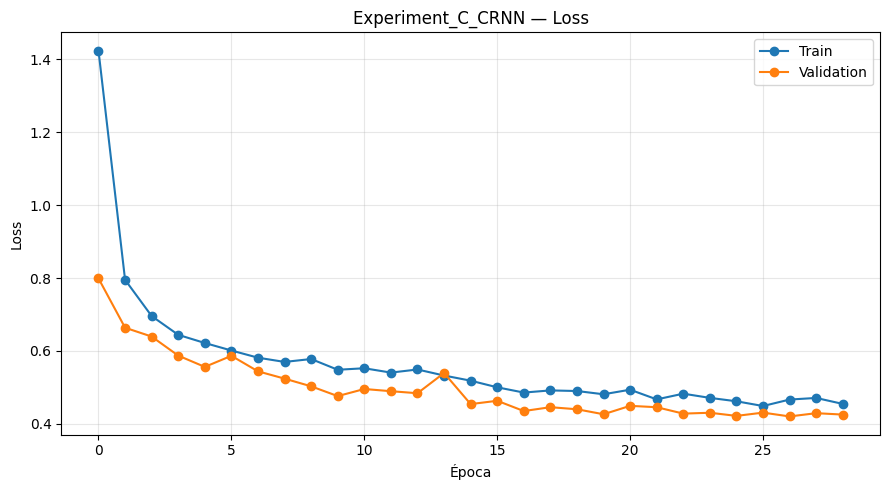
\includegraphics[width=\columnwidth]
{crnn_learning_curves.png}
\caption{Training and validation learning curves of the CRNN model.}
\label{fig:crnn_learning_curves}
\end{figure}
As observed in Fig.~\ref{fig:crnn_confusion_matrix}, the hybrid model correctly classified most samples while reducing several of the errors observed in the CNN1D. Nevertheless, some confusion remained among activities with related motion structures, suggesting that the convolutional compression stage may have removed part of the temporal information required for more precise discrimination.

\subsection{Comparative Analysis}

Table~\ref{tab:model_comparison} summarizes the principal results obtained by the three evaluated architectures. The BiLSTM achieved the highest test accuracy and Macro F1-score, substantially outperforming both convolution-based alternatives. The CRNN obtained the second-highest classification performance, while the CNN1D produced the lowest accuracy but required the shortest training time and the smallest number of trainable parameters.

The difference between Accuracy and Macro F1-score was particularly relevant for the CNN1D and CRNN models. Because the KU-HAR dataset presents an unequal number of samples across activity classes, conventional accuracy is influenced more strongly by the most represented categories. Macro F1-score assigns the same importance to every class and therefore provides a complementary evaluation of performance under class imbalance.

From a computational perspective, the CNN1D required approximately 181 seconds to train, whereas the CRNN required approximately seven minutes. In contrast, the BiLSTM required approximately 1.5 hours, making it nearly 30 times slower than the CNN1D and approximately 13 times slower than the CRNN.

\begin{table*}[!t]
\caption{Comparative Performance of the Evaluated Deep Learning Models}
\label{tab:model_comparison}
\centering
\begin{tabular}{lcccccc}
\hline
Model &
Accuracy &
Balanced Accuracy &
Macro F1 &
Weighted F1 &
Parameters &
Training Time \\
\hline
CNN1D &
82.78\% &
88.86\% &
89.29\% &
83.38\% &
260,754 &
181 s \\

BiLSTM &
\textbf{97.37\%} &
-- &
\textbf{98.08\%} &
-- &
-- &
$\approx$1.5 h \\

CRNN &
85.93\% &
\textbf{90.76\%} &
91.00\% &
86.03\% &
361,106 &
$\approx$7 min \\
\hline
\end{tabular}
\end{table*}

\begin{figure}[!t]
\centering
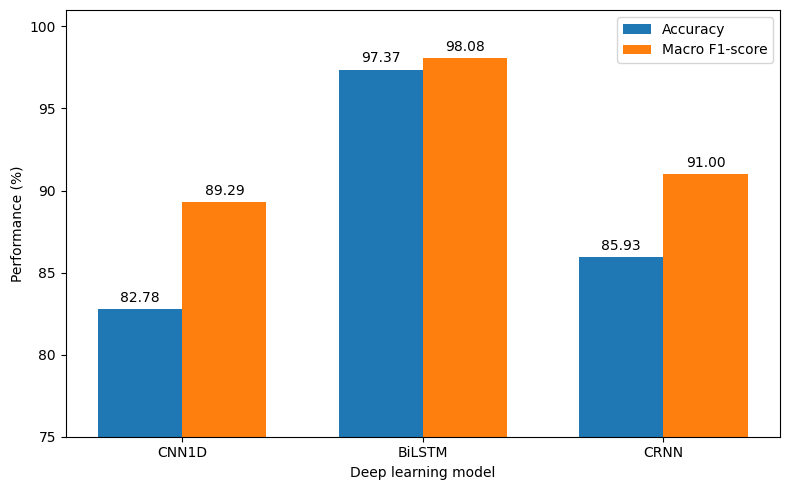
\includegraphics[width=\columnwidth]
{model_performance_comparison.png}
\caption{Comparison of test Accuracy and Macro F1-score among the evaluated models.}
\label{fig:performance_comparison}
\end{figure}

Figure~\ref{fig:performance_comparison} illustrates the difference in classification performance among the evaluated models. The BiLSTM exceeded the CNN1D by 14.59 percentage points in accuracy and exceeded the CRNN by 11.44 percentage points.

\begin{figure}[!t]
\centering
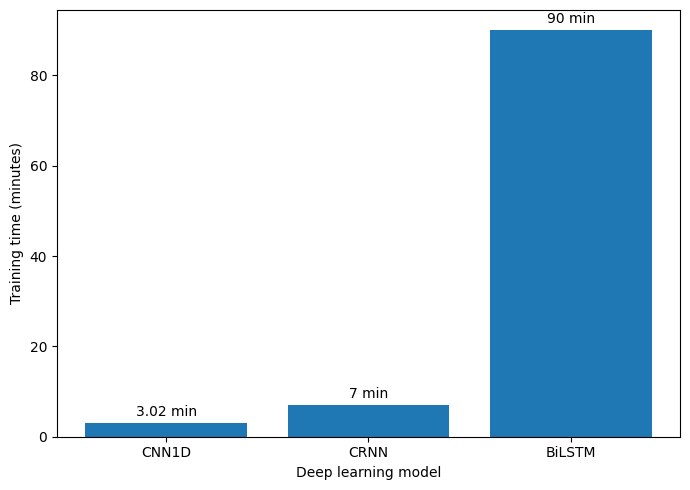
\includegraphics[width=\columnwidth]
{training_time_comparison.png}
\caption{Comparison of the approximate training time required by each architecture.}
\label{fig:training_time}
\end{figure}

As shown in Fig.~\ref{fig:training_time}, the superior predictive performance of the BiLSTM was associated with a considerably higher computational cost. The CNN1D was the fastest architecture, while the CRNN provided an intermediate training time.


\section{Discussion}

The experimental results demonstrate that the three evaluated architectures exhibit distinct strengths depending on the balance between classification performance and computational efficiency. Although all models were capable of learning meaningful representations from the KU-HAR dataset, significant differences were observed in their ability to model temporal dependencies and their associated computational requirements.

\subsection{Performance Analysis}

Among the evaluated architectures, the BiLSTM consistently achieved the highest recognition performance, reaching a test accuracy of 97.37\% and a Macro F1-score of 98.08\%. These results indicate that explicitly modeling temporal dependencies in both forward and backward directions provides a significant advantage for recognizing complex human activities from inertial sensor signals.

Unlike convolutional models, recurrent architectures preserve the temporal order of the complete sequence during feature extraction. This capability is particularly beneficial for HAR because many activities are characterized not only by individual sensor values but also by the evolution of movement over time. Consequently, the BiLSTM was able to distinguish activities with similar instantaneous motion patterns but different temporal dynamics more effectively than the other evaluated models.

\subsection{CNN and CRNN Behavior}

Although the CRNN combined convolutional feature extraction with recurrent processing, its performance remained below that of the BiLSTM. A possible explanation is that the initial convolutional layers compressed part of the temporal information before it reached the recurrent component. While convolution efficiently extracts local motion features, some long-range temporal dependencies may be partially attenuated during pooling operations.

The KU-HAR dataset contains relatively clean and well-segmented activity windows. Under these conditions, directly processing the complete temporal sequence through a BiLSTM appears to preserve richer contextual information than first applying convolutional compression. Consequently, the additional convolutional stage did not provide sufficient complementary information to compensate for the loss of temporal resolution.

\subsection{Computational Efficiency}

The CNN1D obtained the lowest classification accuracy but also required the shortest training time and the smallest number of trainable parameters. This result confirms one of the principal advantages of convolutional architectures: efficient feature extraction with relatively low computational complexity.

Despite its lower predictive performance, the CNN1D achieved an accuracy exceeding 82\%, demonstrating that local temporal patterns alone contain sufficient information to correctly recognize most activities. Therefore, CNN-based architectures remain attractive candidates for resource-constrained environments such as smartphones, wearable devices, and embedded systems, where computational efficiency is often a primary design consideration.

\subsection{Trade-off Between Accuracy and Computational Cost}

An important outcome of this study is the evident trade-off between recognition performance and computational cost. The BiLSTM provided the highest classification accuracy but required approximately 1.5 hours of training, making it nearly thirty times slower than the CNN1D and considerably slower than the CRNN.

Conversely, the CNN1D completed training in approximately three minutes while maintaining competitive performance. The CRNN occupied an intermediate position, requiring approximately seven minutes of training while providing moderate improvements over the CNN1D.

These findings suggest that the optimal architecture depends on the intended application. Systems prioritizing maximum recognition accuracy may benefit from recurrent architectures such as BiLSTM, whereas real-time or embedded applications may favor CNN-based models due to their substantially lower computational requirements.

\subsection{Limitations}

Although the proposed comparison provides valuable insights into the performance of representative deep learning architectures, several limitations should be acknowledged. First, all experiments were conducted using a single publicly available dataset. Consequently, the observed performance may vary when evaluated on datasets collected under different acquisition protocols or sensor configurations.

Second, only three representative architectures were investigated. More recent sequence models based on attention mechanisms or transformer architectures may provide additional improvements in recognition performance while reducing computational complexity.

Finally, inference time and energy consumption were not evaluated in this study. These aspects are particularly relevant for real-time smartphone applications and should be considered in future research.

\begin{table}[!t]
\caption{Summary of the Strengths and Limitations of the Evaluated Models}
\label{tab:discussion}
\centering
\begin{tabular}{lccc}
\hline
Property & CNN1D & BiLSTM & CRNN\\
\hline
Recognition Accuracy & Medium & High & Medium-High\\
Training Time & Low & High & Medium\\
Model Complexity & Low & High & Medium\\
Temporal Modeling & Limited & Excellent & Good\\
Mobile Deployment & Excellent & Limited & Good\\
\hline
\end{tabular}
\end{table}

As summarized in Table~\ref{tab:discussion}, each architecture presents different strengths depending on the requirements of the target application.

\section{Conclusion}

This work presented a comparative evaluation of three deep learning architectures for smartphone-based Human Activity Recognition using the KU-HAR dataset. A one-dimensional Convolutional Neural Network (CNN1D), a Bidirectional Long Short-Term Memory network (BiLSTM), and a hybrid Convolutional Recurrent Neural Network (CRNN) were implemented under identical preprocessing, training, and evaluation conditions to ensure a fair comparison.

Among the evaluated models, the BiLSTM achieved the highest predictive performance, reaching a test accuracy of 97.37\% and a Macro F1-score of 98.08\%. These results demonstrate the importance of explicitly modeling long-term temporal dependencies when classifying multivariate inertial sensor signals. In contrast, the CNN1D provided the shortest training time and the lowest computational complexity, making it a suitable alternative for applications where computational resources are limited. The CRNN offered an intermediate solution, improving classification performance over the CNN1D while maintaining a substantially lower computational cost than the BiLSTM.

Overall, the experimental results confirm that selecting an appropriate architecture for Human Activity Recognition requires balancing predictive performance and computational efficiency according to the target application. While recurrent architectures maximize recognition accuracy, convolutional approaches remain attractive for real-time and embedded implementations due to their lower computational requirements.

Future research will focus on evaluating more recent sequence-learning architectures, including Transformer-based and attention-based models, to determine whether higher recognition accuracy can be achieved without substantially increasing computational cost. In addition, future studies should investigate cross-subject generalization, real-time inference performance, and energy consumption on mobile and embedded devices to better assess the practical deployment of Human Activity Recognition systems.

\bibliographystyle{IEEEtran}
\bibliography{references}







%\subsection{Subsection Heading Here}
%Subsection text here.

% needed in second column of first page if using \IEEEpubid
%\IEEEpubidadjcol

%\subsubsection{Subsubsection Heading Here}
%Subsubsection text here.


%\section{Resultados}

%referencia a tabla \ref{table:example}
% Ejemplo de tabla
%\begin{table}[h]
%    \centering
%    \caption{Ejemplo de tabla.}
%    \label{table:example}
%    \begin{tabular}{|c|c|c|}
%        \hline
%        \textbf{Columna 1} & \textbf{Columna 2} & \textbf{Columna 3} \\
%        \hline
%        Dato 1 & Dato 2 & Dato 3 \\
%        \hline
%        Dato 4 & Dato 5 & Dato 6 \\
%        \hline
%        Dato 7 & Dato 8 & Dato 9 \\
%        \hline
%    \end{tabular}
%\end{table}

% Ejemplo de figura
%\begin{figure}[ht]
%    \centering
%    
\includegraphics[scale=0.17]{AIlogo.jpg}
%    \caption{Ejemplo de figura.}
%    \label{fig:example}
%\end{figure}

% An example of a floating figure using the graphicx package.
% Note that \label must occur AFTER (or within) \caption.
% For figures, \caption should occur after the \includegraphics.
% Note that IEEEtran v1.7 and later has special internal code that
% is designed to preserve the operation of \label within \caption
% even when the captionsoff option is in effect. However, because
% of issues like this, it may be the safest practice to put all your
% \label just after \caption rather than within \caption{}.
%
% Reminder: the "draftcls" or "draftclsnofoot", not "draft", class
% option should be used if it is desired that the figures are to be
% displayed while in draft mode.
%
%\begin{figure}[!t]
%\centering
%\includegraphics[width=2.5in]{myfigure}
% where an .eps filename suffix will be assumed under latex, 
% and a .pdf suffix will be assumed for pdflatex; or what has been declared
% via \DeclareGraphicsExtensions.
%\caption{Simulation results for the network.}
%\label{fig_sim}
%\end{figure}

% Note that the IEEE typically puts floats only at the top, even when this
% results in a large percentage of a column being occupied by floats.


% An example of a double column floating figure using two subfigures.
% (The subfig.sty package must be loaded for this to work.)
% The subfigure \label commands are set within each subfloat command,
% and the \label for the overall figure must come after \caption.
% \hfil is used as a separator to get equal spacing.
% Watch out that the combined width of all the subfigures on a 
% line do not exceed the text width or a line break will occur.
%
%\begin{figure*}[!t]
%\centering
%\subfloat[Case I]{\includegraphics[width=2.5in]{box}%
%\label{fig_first_case}}
%\hfil
%\subfloat[Case II]{\includegraphics[width=2.5in]{box}%
%\label{fig_second_case}}
%\caption{Simulation results for the network.}
%\label{fig_sim}
%\end{figure*}
%
% Note that often IEEE papers with subfigures do not employ subfigure
% captions (using the optional argument to \subfloat[]), but instead will
% reference/describe all of them (a), (b), etc., within the main caption.
% Be aware that for subfig.sty to generate the (a), (b), etc., subfigure
% labels, the optional argument to \subfloat must be present. If a
% subcaption is not desired, just leave its contents blank,
% e.g., \subfloat[].


% An example of a floating table. Note that, for IEEE style tables, the
% \caption command should come BEFORE the table and, given that table
% captions serve much like titles, are usually capitalized except for words
% such as a, an, and, as, at, but, by, for, in, nor, of, on, or, the, to
% and up, which are usually not capitalized unless they are the first or
% last word of the caption. Table text will default to \footnotesize as
% the IEEE normally uses this smaller font for tables.
% The \label must come after \caption as always.
%
%\begin{table}[!t]
%% increase table row spacing, adjust to taste
%\renewcommand{\arraystretch}{1.3}
% if using array.sty, it might be a good idea to tweak the value of
% \extrarowheight as needed to properly center the text within the cells
%\caption{An Example of a Table}
%\label{table_example}
%\centering
%% Some packages, such as MDW tools, offer better commands for making tables
%% than the plain LaTeX2e tabular which is used here.
%\begin{tabular}{|c||c|}
%\hline
%One & Two\\
%\hline
%Three & Four\\
%\hline
%\end{tabular}
%\end{table}


% Note that the IEEE does not put floats in the very first column
% - or typically anywhere on the first page for that matter. Also,
% in-text middle ("here") positioning is typically not used, but it
% is allowed and encouraged for Computer Society conferences (but
% not Computer Society journals). Most IEEE journals/conferences use
% top floats exclusively. 
% Note that, LaTeX2e, unlike IEEE journals/conferences, places
% footnotes above bottom floats. This can be corrected via the
% \fnbelowfloat command of the stfloats package.


%\section{Conclusion}
%The conclusion goes here.\cite{IEEEexample:articledualmonths,IEEEexample:babel}


% if have a single appendix:
%\appendix[Proof of the Zonklar Equations]
% or
%\appendix  % for no appendix heading
% do not use \section anymore after \appendix, only \section*
% is possibly needed

% use appendices with more than one appendix
% then use \section to start each appendix
% you must declare a \section before using any
% \subsection or using \label (\appendices by itself
% starts a section numbered zero.)
%


%\appendices
%\section{Proof of the First Zonklar Equation}
%Appendix one text goes here.

% you can choose not to have a title for an appendix
% if you want by leaving the argument blank
%\section{Appendix title two goes here}
%Appendix two text goes here.


% use section* for acknowledgment
%\section*{Acknowledgment}


%The authors would like to thank... 


% Can use something like this to put references on a page
% by themselves when using endfloat and the captionsoff option.
\ifCLASSOPTIONcaptionsoff
  \newpage
\fi


% trigger a \newpage just before the given reference
% number - used to balance the columns on the last page
% adjust value as needed - may need to be readjusted if
% the document is modified later
%\IEEEtriggeratref{8}
% The "triggered" command can be changed if desired:
%\IEEEtriggercmd{\enlargethispage{-5in}}

% references section

% can use a bibliography generated by BibTeX as a .bbl file
% BibTeX documentation can be easily obtained at:
% http://mirror.ctan.org/biblio/bibtex/contrib/doc/
% The IEEEtran BibTeX style support page is at:
% http://www.michaelshell.org/tex/ieeetran/bibtex/
\bibliographystyle{IEEEtran}
% argument is your BibTeX string definitions and bibliography database(s)
\bibliography{IEEEabrv,./bibtex/bib/IEEEexample.bib}
%
% <OR> manually copy in the resultant .bbl file
% set second argument of \begin to the number of references
% (used to reserve space for the reference number labels box)
%\begin{thebibliography}{1}

%\bibitem{IEEEhowto:kopka}
%H.~Kopka and P.~W. Daly, \emph{A Guide to \LaTeX}, 3rd~ed.\hskip 1em plus
%  0.5em minus 0.4em\relax Harlow, England: Addison-Wesley, 1999.

%\end{thebibliography}

% biography section
% 
% If you have an EPS/PDF photo (graphicx package needed) extra braces are
% needed around the contents of the optional argument to biography to prevent
% the LaTeX parser from getting confused when it sees the complicated
% \includegraphics command within an optional argument. (You could create
% your own custom macro containing the \includegraphics command to make things
% simpler here.)
% \begin{IEEEbiography}[{\includegraphics[width=1in,height=1.25in,clip,keepaspectratio]{mshell}}]{Michael Shell}
% or if you just want to reserve a space for a photo:

%\begin{IEEEbiography}{Michael Shell}
%Biography text here.
%\end{IEEEbiography}

% if you will not have a photo at all:
%\begin{IEEEbiographynophoto}{John Doe}
%Biography text here.
%\end{IEEEbiographynophoto}

%\begin{IEEEbiographynophoto}{Jane Doe}
%Biography text here.
%\end{IEEEbiographynophoto}

% insert where needed to balance the two columns on the last page with
% biographies
%\newpage

%\begin{IEEEbiographynophoto}{Joshua Reinoso}
%Biography text here.
%\end{IEEEbiographynophoto}

% You can push biographies down or up by placing
% a \vfill before or after them. The appropriate
% use of \vfill depends on what kind of text is
% on the last page and whether or not the columns
% are being equalized.

%\vfill

% Can be used to pull up biographies so that the bottom of the last one
% is flush with the other column.
%\enlargethispage{-5in}


% that's all folks
\end{document}